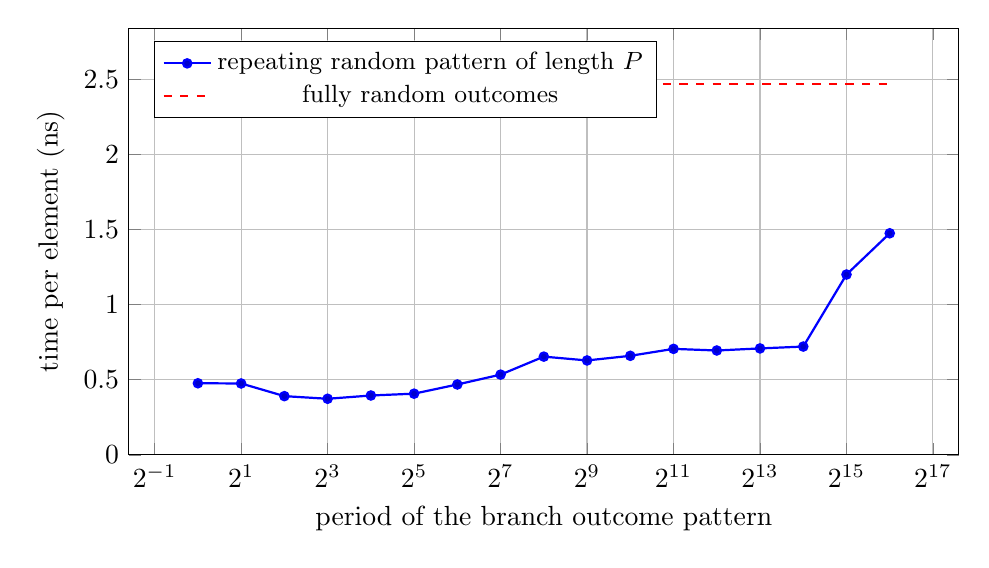
\begin{tikzpicture}
\begin{axis}[width=\textwidth, height=7cm, xmode=log, log basis x=2, xlabel={period of the branch outcome pattern}, ylabel={time per element (ns)}, grid=major, ymin=0, ymax=2.84,
  legend pos=north west, legend style={font=\small}]
\addplot+[mark=*, mark size=1.5pt, thick] coordinates {(1,0.4767) (2,0.4753) (4,0.391) (8,0.3734) (16,0.3952) (32,0.4074) (64,0.4686) (128,0.5342) (256,0.654) (512,0.6285) (1024,0.6594) (2048,0.7056) (4096,0.6948) (8192,0.7086) (16384,0.7209) (32768,1.2005) (65536,1.475)};
\addlegendentry{repeating random pattern of length $P$}
\addplot[red, dashed, thick, domain=1:65536] {2.4690};
\addlegendentry{fully random outcomes}
\end{axis}
\end{tikzpicture}